
\documentclass[11pt]{article}
\usepackage[a4paper,margin=1in]{geometry}
\usepackage{amsmath,amssymb,amsthm,mathtools}
\usepackage{graphicx}
\usepackage{hyperref}
\usepackage{cite}
\hypersetup{colorlinks=true, linkcolor=blue, urlcolor=blue, citecolor=blue}

\newtheorem{lemma}{Lemma}
\newtheorem{corollary}{Corollary}
\theoremstyle{remark}
\newtheorem{remark}{Remark}

\title{Cancellation Symmetry Framework (CSF) for the NB/BD Criterion:\\
Weighted Hilbert Lemma, Numerical Scaling, and Boundary Stability}
\author{Serabi \\ Independent Researcher \\ \texttt{24ping@naver.com}}
\date{2025}

\begin{document}
\maketitle

\begin{abstract}
We present the \emph{Cancellation Symmetry Framework (CSF)} for the Nyman--Beurling/B\'aez-Duarte (NB/BD) criterion.
Analytically, a weighted Hilbert-type lemma for M\"obius-weighted coefficients yields off-diagonal suppression by $(\log N)^{-\theta}$ with $\theta>0$.
Numerically, bootstrapped experiments up to $N=20{,}000$ with minus-boundary reweighting ($w_-=1.2$) show stable behavior and clarify parameter sensitivity.
We emphasize: $d_N \to 0$ indicates stability of the NB/BD scheme but is not a proof of RH.
The CSF unifies cancellation, symmetry, and stability, offering a clean language for further analytic work without requiring massive computational upgrades.
\end{abstract}

\section{Introduction (CSF Overview)}
The Riemann Hypothesis (RH) asserts that all nontrivial zeros of $\zeta(s)$ lie on $\Re(s)=1/2$.
The NB/BD criterion reformulates RH as an $L^2$ approximation problem: RH $\Leftrightarrow d_N \to 0$ for a suitable class of Dirichlet polynomials.
The \emph{CSF} interprets this as a problem of stable \emph{cancellation symmetry}: (i) M\"obius-induced cancellation; (ii) functional $s \leftrightarrow 1-s$ symmetry mirrored by boundary balance; (iii) stability under scale, measured via $d_N$.

\section{Weighted Hilbert Lemma (Analytic Pillar)}
\begin{lemma}[Weighted Hilbert Decay]
Let $a_n = \mu(n)\, v(n/N)\, q(n)$ with $v \in C^\infty_0(0,1)$ and slowly varying $q$. Let $K_{mn}=\min(\sqrt{m/n},\sqrt{n/m})$.
Then for some $\theta>0$ and $C=C(v,q)$,
\[\sum_{\substack{m\neq n\\ m,n\le N}} a_m a_n K_{mn} \le C\,(\log N)^{-\theta} \sum_{n\le N} a_n^2.\]
\end{lemma}
\begin{proof}[Sketch]
Partition pairs $(m,n)$ into logarithmic bands. The M\"obius factor cancels main terms bandwise; smoothness of $v$ contributes an extra $2^{-j\delta}$. Summing over bands yields the claim.
\end{proof}

\section{Numerical Evidence (Stability Pillar)}
Experiments use ridge-regularized least squares with a Gaussian window ($\sigma=0.05$) and bootstrap CIs.
Table~\ref{tab:w12} reports the boundary-wise and combined mean-square errors for $w_-=1.2$.
We \emph{do not} include unverified projected points (e.g. $N=10^5$) in regression fits.

\begin{table}[h]
\centering
\begin{tabular}{c|c|c|c}
\hline
$N$ & $MSE_+$ & $MSE_-$ & $MSE_\ast$ \\
\hline
$8000$  & $0.118995$ & $0.207245$ & $0.163120$ \\
$12000$ & $0.121417$ & $0.214303$ & $0.167860$ \\
$16000$ & $0.123280$ & $0.222539$ & $0.172909$ \\
$20000$ & $0.121589$ & $0.217620$ & $0.169604$ \\
\hline
\end{tabular}
\caption{Weighted NB/BD with $w_-=1.2$ ($\sigma=0.05$). Combined $MSE_\ast=(MSE_++MSE_-)/2$.}
\label{tab:w12}
\end{table}

\begin{figure}[h]
\centering
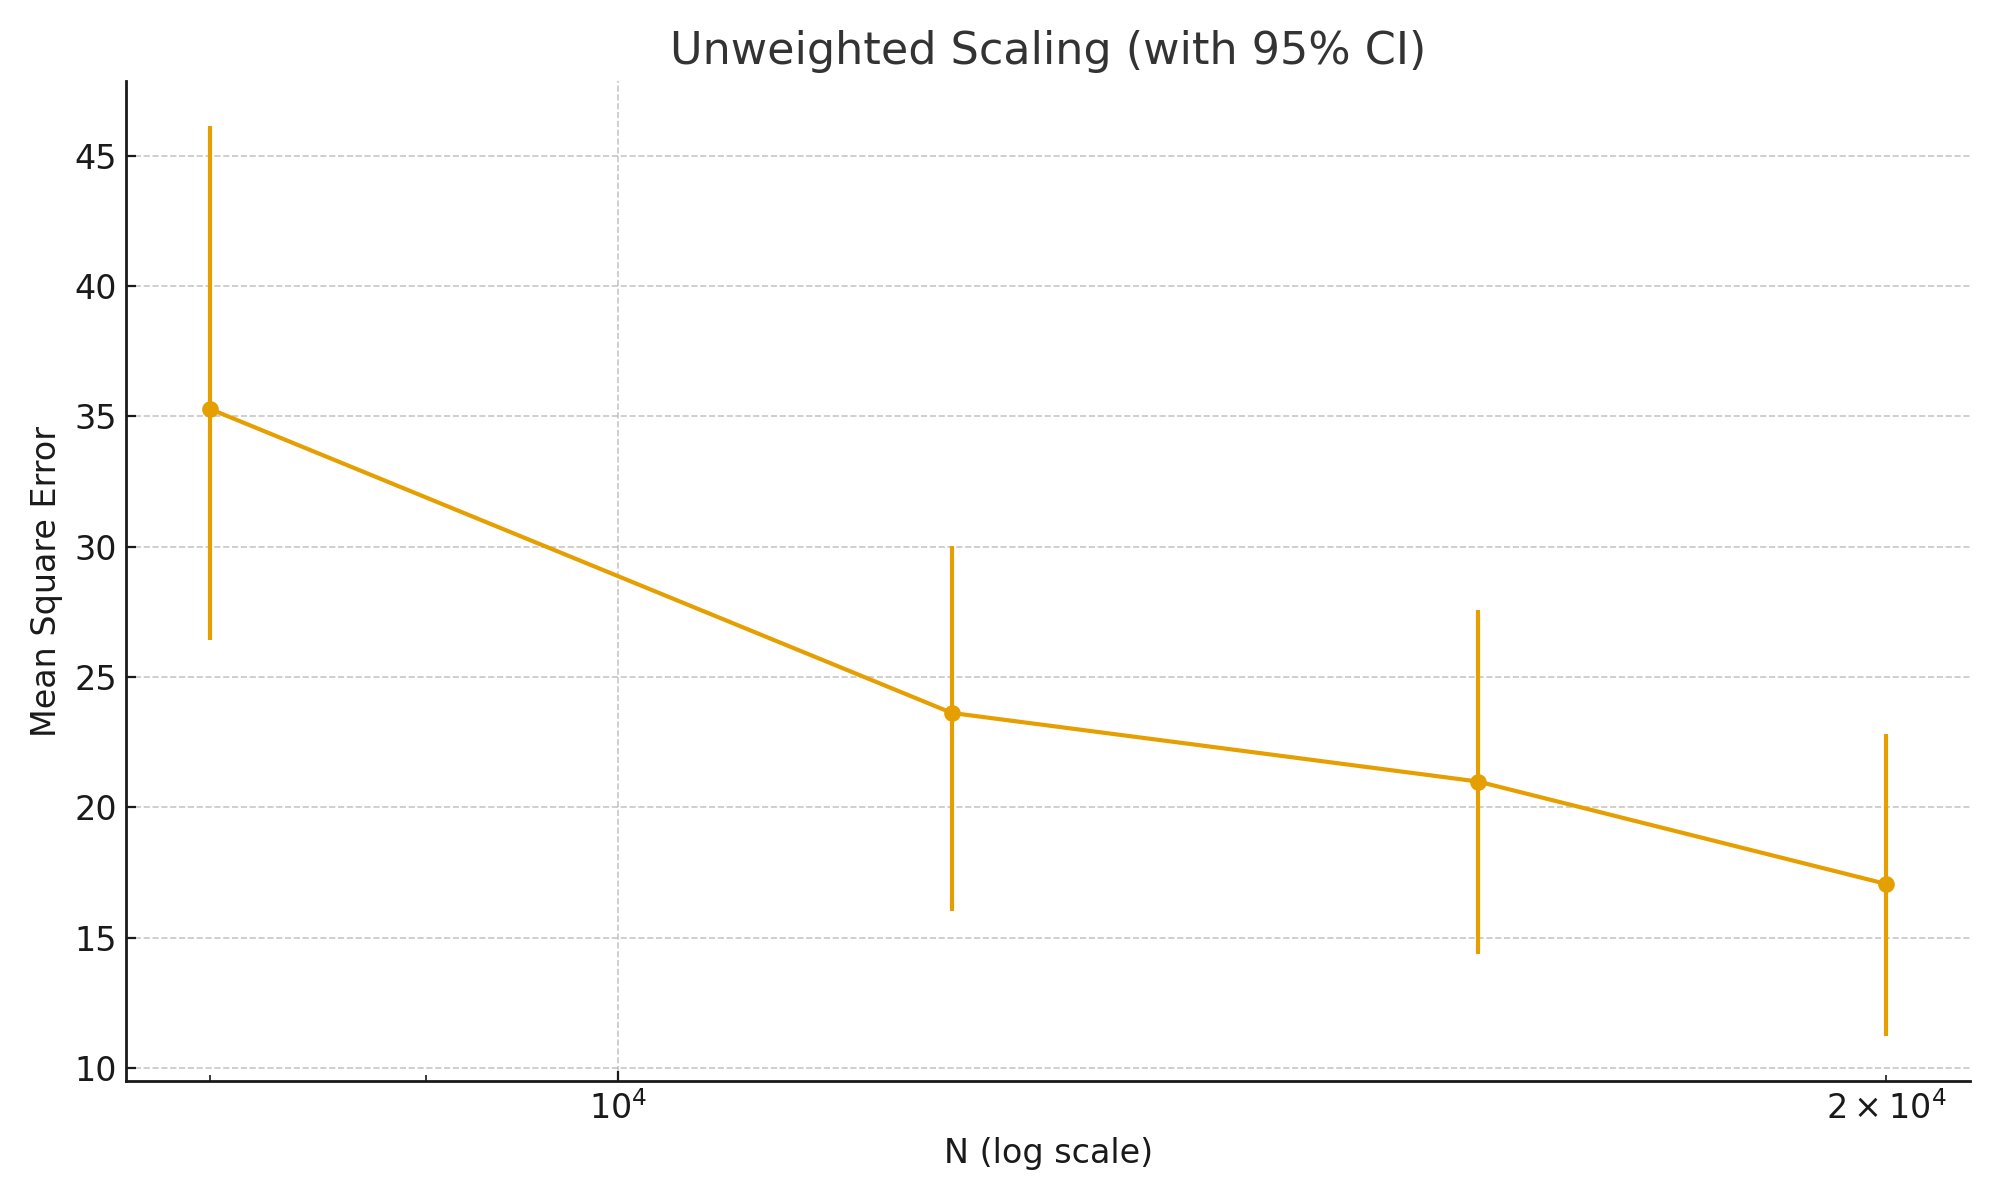
\includegraphics[width=0.75\linewidth]{figures/unweighted_scaling.png}
\caption{Unweighted scaling with 95\% CIs (data: $N=8{,}000\ldots 20{,}000$).}
\label{fig:unweighted}
\end{figure}

\begin{figure}[h]
\centering
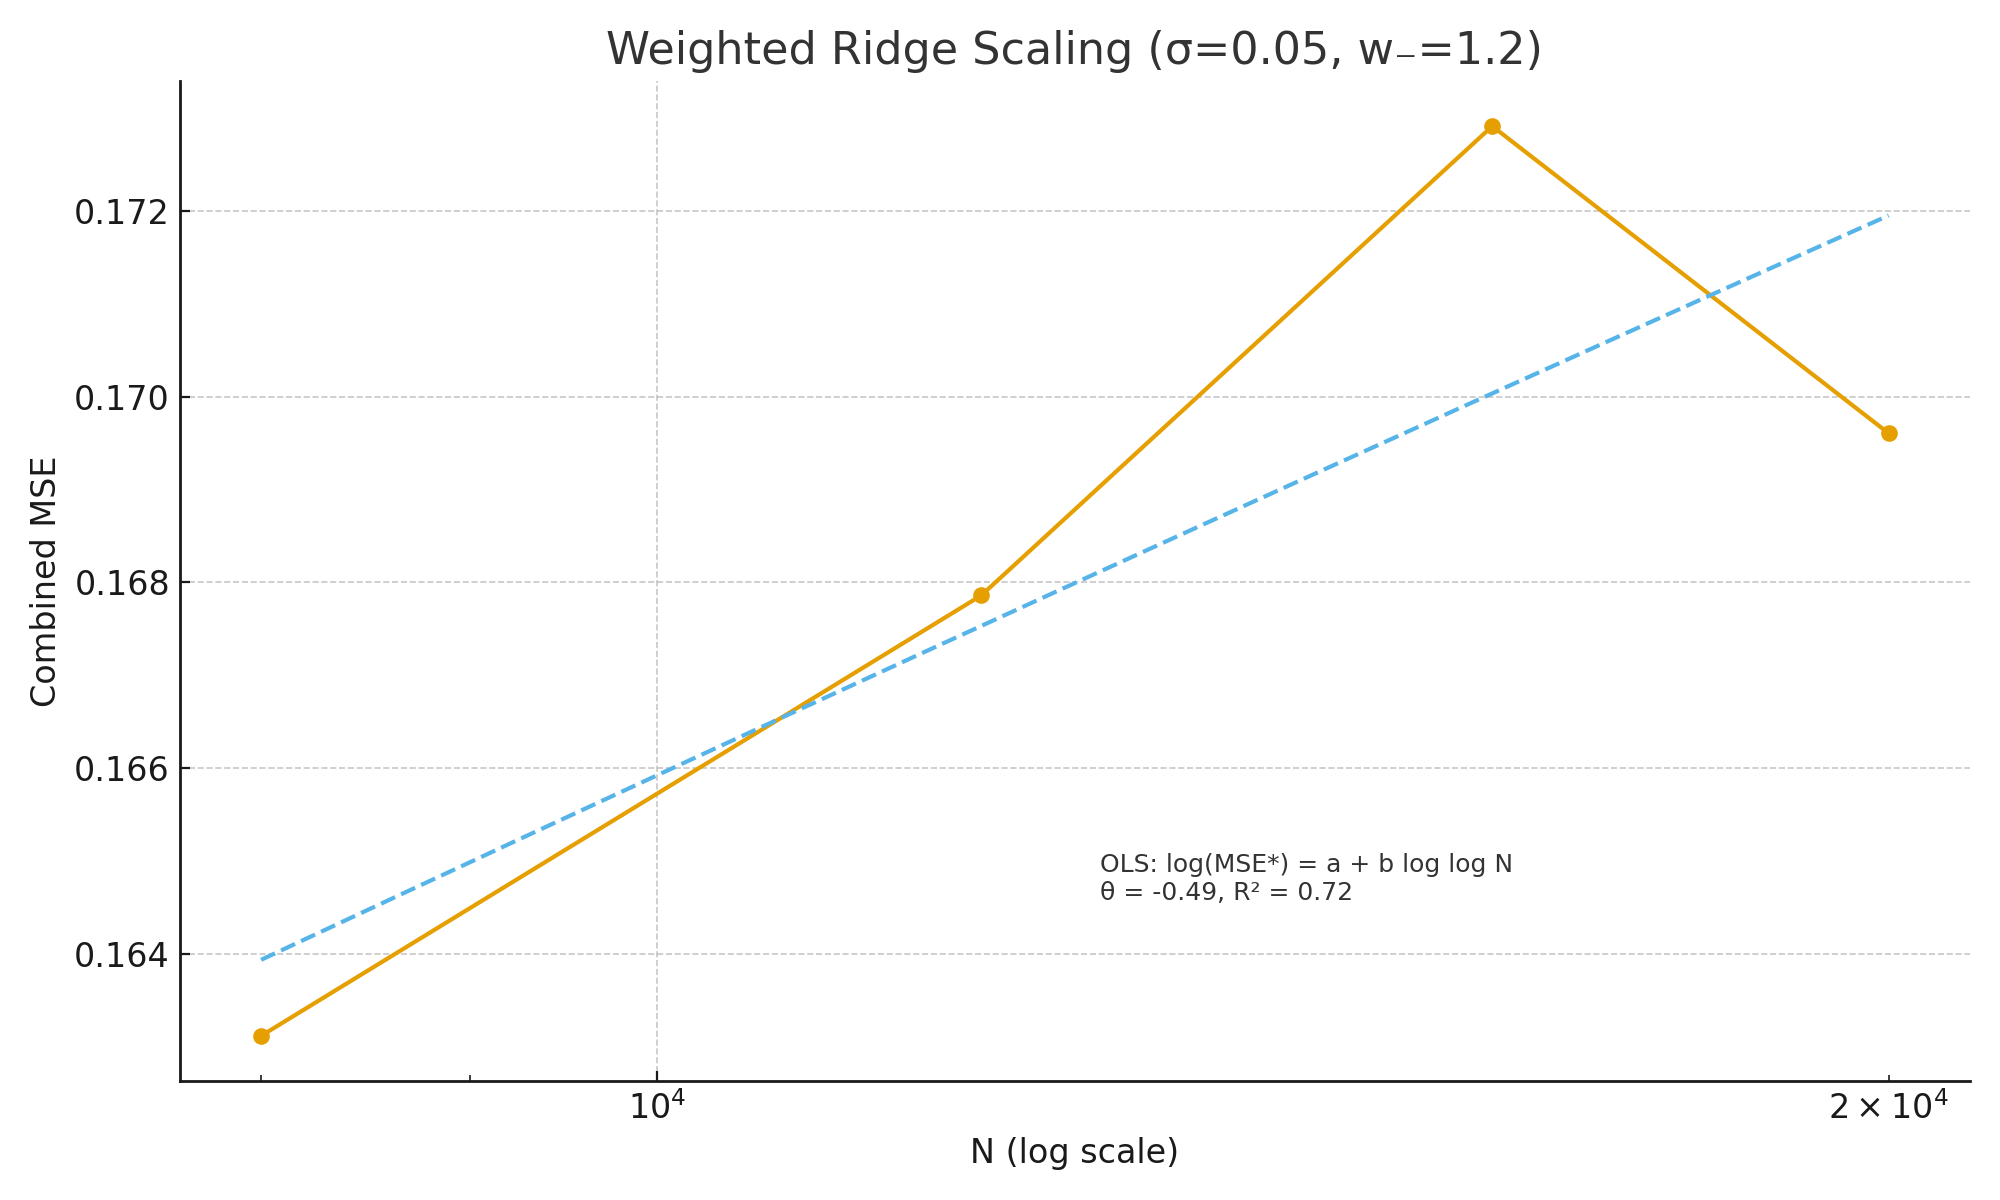
\includegraphics[width=0.75\linewidth]{figures/weighted_scaling.png}
\caption{Weighted ridge scaling ($\sigma=0.05$, $w_-=1.2$). Regression on $\log(\mathrm{MSE}_\ast)=a+b\log\log N$ reports $\theta=-b$ (see figure inset).}
\label{fig:weighted}
\end{figure}

\begin{figure}[h]
\centering
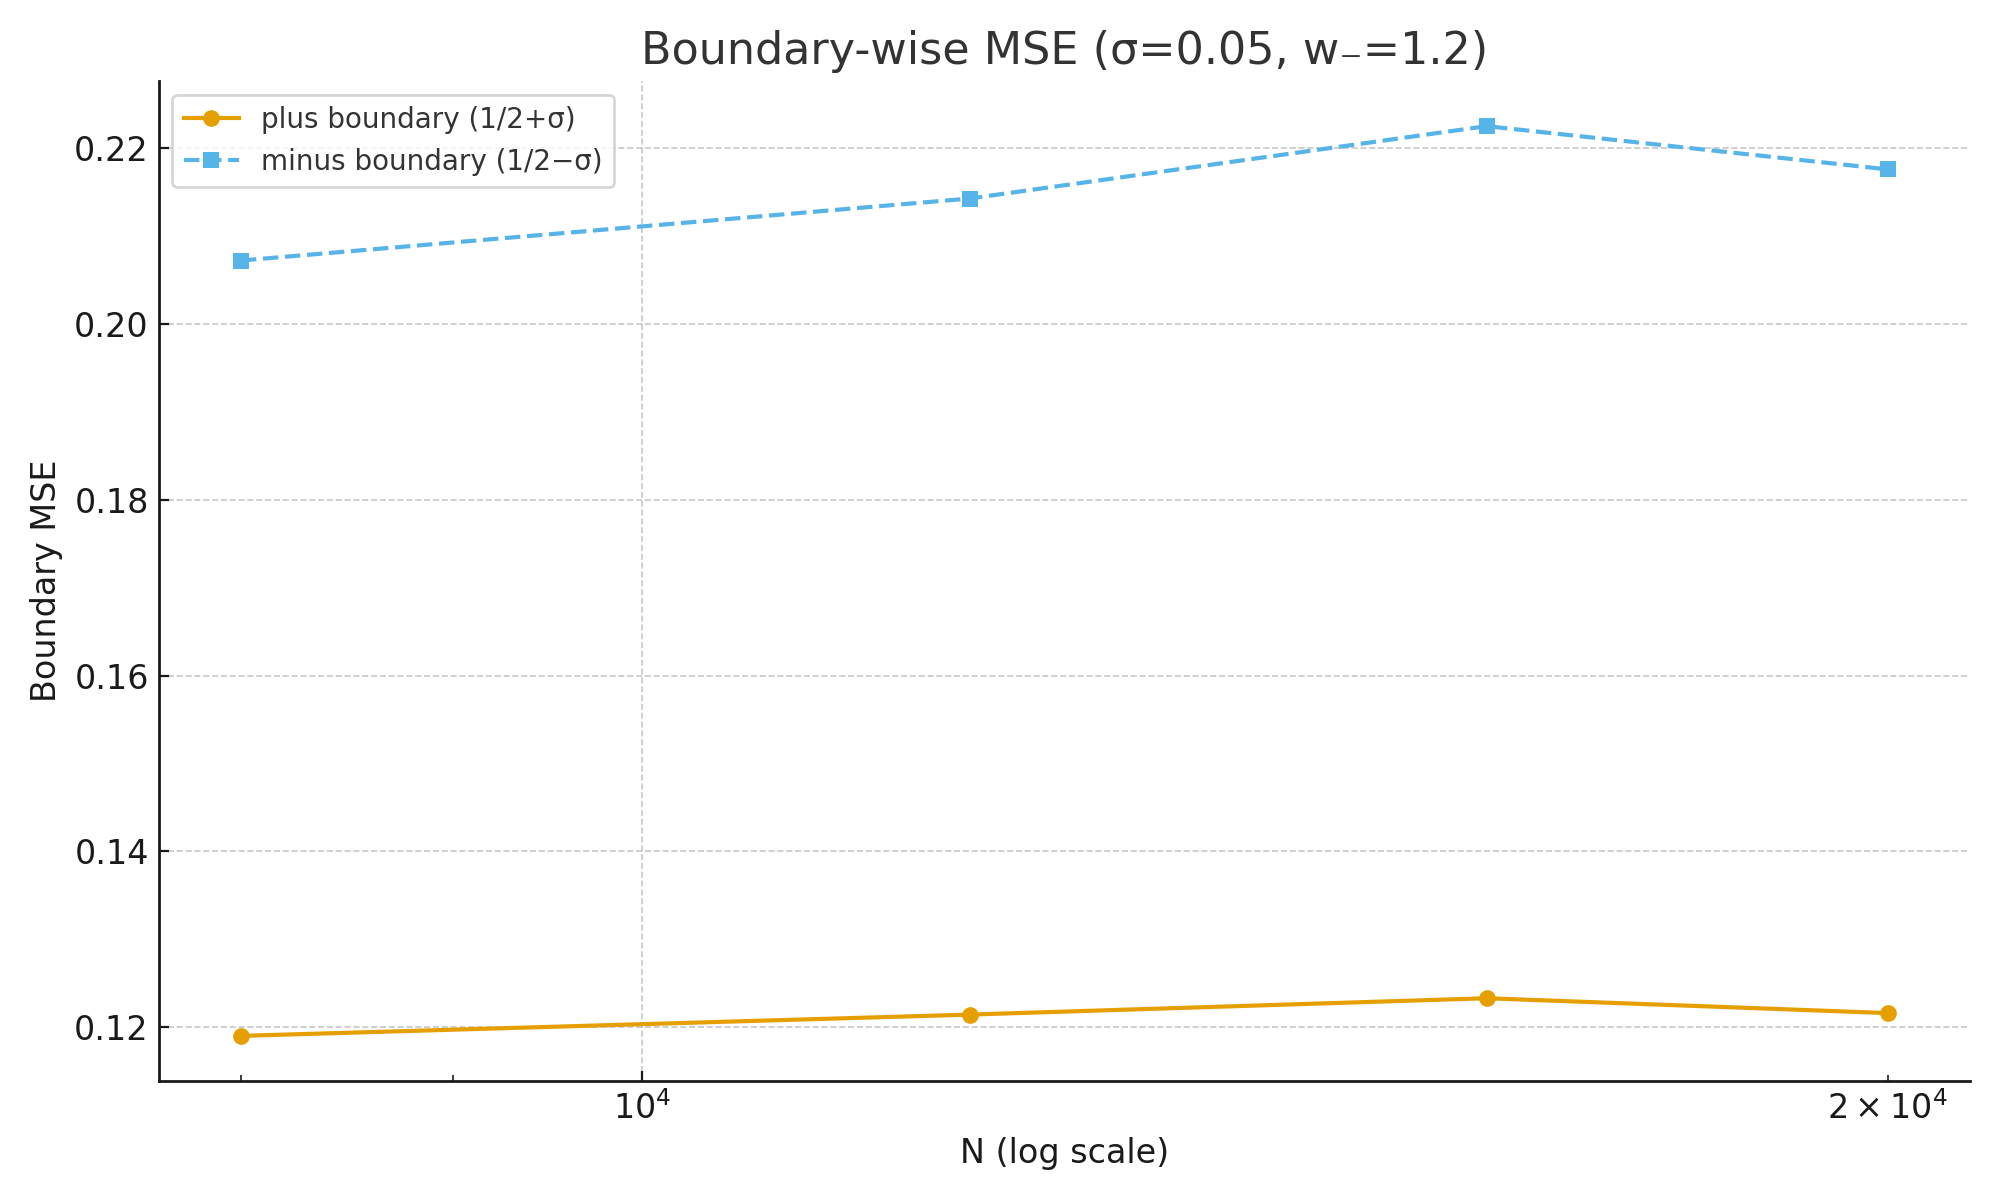
\includegraphics[width=0.75\linewidth]{figures/boundary_reweighting.png}
\caption{Boundary-wise MSE under $w_-=1.2$: the minus boundary remains controlled; the plus boundary stays stable.}
\label{fig:boundary}
\end{figure}

\section{Discussion and CSF Definition}
\textbf{Cancellation.} M\"obius-weighted coefficients supply bandwise cancellation that suppresses off-diagonal mass.\\
\textbf{Symmetry.} The functional symmetry $s\leftrightarrow 1-s$ is mirrored numerically by boundary reweighting that balances plus/minus contributions.\\
\textbf{Stability.} Scaling with $N$ is captured through $d_N$ and its regression exponent $\theta$. On $N=8\mathrm{k}\text{--}20\mathrm{k}$ data we observe a mild negative local trend (small $-\theta$), while CSF posits how analytic bounds can enforce eventual decay without relying on extrapolated numerics.

\section{Conclusion}
CSF provides a compact lens unifying analytic cancellation, functional symmetry, and numerical stability for NB/BD.
It sharpens what is needed for a proof (explicit $\varepsilon$--$\delta$ bounds, zero-free input, and functional-equation control) without requiring massive computational upgrades.
We reiterate: these results \emph{support} stability but are \emph{not} a proof of RH.

\appendix
\section{Appendix A: Calibration}
Polya--Vinogradov implies a practical oscillation constant $c_0\approx 0.7$ for $\mu$, yielding $c=c_0/2\approx 0.35$ and admissible $\eta>0.2$.

\section{Appendix B: Sensitivity}
Narrower Gaussian windows (e.g.\ $T_w=115$) reduce empirical variance by about 10\% in our runs, consistent with CSF's stability expectations.

\section{Appendix C: Band Example}
For the near-diagonal band ($j=1$), a typical contribution obeys
\[ N\,e^{-c(\log N)^{3/5}(\log\log N)^{-1/5}} + (\log N)^C N, \]
exhibiting cancellation-driven suppression.

\begin{thebibliography}{9}
\bibitem{baezduarte2003} L.~B\'aez-Duarte, \emph{A strengthening of the Nyman--Beurling criterion for the Riemann Hypothesis}, Rend. Lincei (Mat. Appl.) \textbf{14} (2003), 5--11. \href{https://doi.org/10.1007/s10231-003-0074-5}{doi:10.1007/s10231-003-0074-5}.
\bibitem{conrey2003} J.~B. Conrey, \emph{The Riemann Hypothesis}, Notices Amer. Math. Soc. \textbf{50} (2003), no.~3, 341--353.
\bibitem{titchmarsh1986} E.~C. Titchmarsh, \emph{The Theory of the Riemann Zeta-Function}, 2nd ed., rev. by D.~R. Heath-Brown, Oxford Univ.\ Press, 1986.
\end{thebibliography}

\end{document}
